\chapter{Asymptotické vlastnosti a souvislost s nebayesiánskými\\ metodami}

\section{Normální aproximace aposteriorního rozdělení}

\subsection{Normální aproximace aposteriorního sdruženého rozdělení}

Jestliže je aposteriorní rozdělení $p(\theta|y)$ unimodální a přibližně symetrické, můžeme ho aproximovat pomocí normální rozdělení, tj. logaritmus aposteriorního rozdělení aproximujeme kvadratickou funkcí parametru $\theta$.

Taylorovým rozvojem $\ln(p(y|\theta))$ centrovaným na aposteriorní mód $\hat{\theta}$ získáváme
\begin{equation}
\ln\big(p(\theta|y)\big) = \ln\big(p(\hat{\theta}|y)\big) + \frac{1}{2}(\theta - \hat{\theta})^T \Big[\frac{d^2}{d \theta^2}\ln\big(p(\theta|y)\big)\Big]_{\theta = \hat{\theta}}(\theta - \hat{\theta}) + ...,
\end{equation}
kde lineární člen rozvoje je nulový, protože derivace pravděpodobnostního rozdělení v jeho módu je rovna nule. Vyšší členy rozvoje můžeme vzhledem k jejich kvadratické formě zanedbat, pokud je $\theta$ dostatečně blízko $\hat{\theta}$ a $n$ dostatečně velké.

První člen rozvoje (4.1) je konstantní a druhý člen je proporcionální logaritmu normálního rozdělení, což vede k aproximaci
\begin{equation}
p(\theta | y) \approx N(\hat{\theta}, [I(\hat{\theta})]^{-1}),
\end{equation}
kde $I(\theta)$ je
\begin{equation}
I(\theta) = - \frac{d^2}{d \theta^2} \ln(p(\theta|y)).
\end{equation}
Jestliže se mód aposteriorního rozdělení $\hat{\theta}$ nachází uvnitř parametrového prostoru, pak je matice $I(\hat{\theta})$ pozitivně definitní.

\subsubsection{Ilustrativní příklad - normální rozdělení s neznámou střední hodnotou a rozptylem}

Nechť $(y_1,..., y_n)$ jsou nezávislá pozorování z $N(\mu, \sigma^2)$ a předpokládejme apriorní uniformní rozdělení pro parametry $(\mu, \ln(\sigma))$. Abychom mohli zkonstruovat výše uvedenou aproximaci, potřebujeme druhou derivaci logaritmu aposteriorního rozdělení,
\begin{equation}
\ln\big(p(\mu, \ln(\sigma)|y)\big) = \textit{konstanta} - n \ln(\sigma) - \frac{1}{2 \sigma^2}\big((n - 1)s^2 + n(\overline{y} - \mu)\big).
\end{equation}
První derivace mají podobu
\begin{equation}
\frac{d}{d \mu} \ln\big(p(\mu, \ln(\sigma)|y)\big) = \frac{n(\overline{y} - \mu)}{\sigma^2},
\end{equation}
\begin{equation}
\frac{d}{d\big(\ln(\sigma)\big)} \ln\big(p(\mu, \ln(\sigma)|y)\big) = -n + \frac{(n - 1)s^2 + n(\overline{y} - \mu)^2}{\sigma^2},
\end{equation}
z nichž lze s pomocí vztahů $\frac{d}{d \mu} = 0$ a $\frac{d}{d(\ln(\sigma))} = 0$ vypočíst mód
\begin{equation}
\big(\hat{\mu}, \ln(\hat{\sigma})\big) = \Big(\overline{y}, \ln\Big(\sqrt{\frac{n - 1}{n}}s\Big)\Big).
\end{equation}
Druhé derivace logaritmu aposteriorního rozdělení jsou pak
\begin{equation}
\frac{d^2}{d \mu^2} \ln\big(p(\mu, \ln(\sigma)|y)\big) = - \frac{n}{\sigma^2},
\end{equation}
\begin{equation}
\frac{d^2}{d \mu d\big(\ln(\sigma)\big)} \ln\big(\mu, \ln(\sigma)|y\big) = -2n \frac{\overline{y} - \mu}{\sigma^2},
\end{equation}
\begin{equation}
\frac{d^2}{d\big(\ln(\sigma)\big)^2}\ln\big(p(\mu, \ln(\sigma)|y)\big) = -\frac{2}{\sigma^2}\big((n - 1)s^2 + n(\overline{y} - \mu)^2 \big).
\end{equation}
Matice druhých derivací v módu je tak
\begin{equation}
\begin{bmatrix}
-n / \hat{\sigma}^2 & 0\\
0 & -2n\\
\end{bmatrix}.
\end{equation}
Pomocí (4.2) tak lze aposteriorní rozdělení aproximovat jako
\begin{equation}
p\big(\mu, \ln(\sigma)|y \big) \approx N \Big(\begin{bmatrix}\mu \\ \ln(\sigma) \end{bmatrix} \Bigm| \begin{bmatrix}\overline{y} \\ \ln(\hat{\sigma}) \end{bmatrix},  \begin{bmatrix}\hat{\sigma}^2 / n & 0\\ 0 & 1 / (2n) \end{bmatrix}\Big).
\end{equation}

Pokud bychom aproximaci konstruovali s pomocí $p(\mu, \sigma^2)$ namísto $p\big(\mu, \ln(\sigma)\big)$, pak bychom matici obsahující derivace druhého řádu násobili Jakobiánem transformační matice z $\ln(\sigma)$ na $\sigma^2$. To by vedlo je změně módu na $\hat{\sigma}^2 = \frac{n}{n + 2}\hat{\sigma}^2$. Obě komponenty parametru $(\mu, \sigma^2)$ by byly rámci aproximace aposteriorního rozdělení stále nezávislé a platilo by $p(\sigma^2 | y) \approx N\big(\sigma^2| \tilde{\sigma}^2, 2 \tilde{\sigma}^4 / (n + 2)\big)$.

\subsection{Interpretace aposteriorního rozdělení s ohledem na jeho maximum}

Kromě aproximace lze vícerozměrné normální rozdělení použít také při interpretaci konturových grafů (contour plots). V případě $d$-rozměrného normálního rozdělení je totiž logaritmus jeho hustoty pravděpodobnosti roven součtu konstanty a $\chi_d^2$ rozdělení vyděleného členem $-2$. Např. 95\% kvantil $\chi_{10}^2$ rozdělení je roven 18.31. Pokud má tedy námi řešený problém $d = 10$ parametrů, pak je 95\% aposteriorní pravděpodobnostní masy spojeno s hodnotami parametru $\theta$, pro které je $p(\theta|y)$ alespoň $e^{-18.31 / 2} = 1.1 \cdot 10^{-4}$ krát pravděpodobnostní hustota v módu. Podobně pro $d = 2$ parametrů odpovídá 95\% aposteriorní pravděpodobnostní masy přibližně hustotě $e^{-5.99 / 2} = 0.05$ a více relativně vzhledem k módu.

\subsection{Předpoklad normality}

Pokud je $n$ dostatečně veliké, často se implicitně předpokládá, že aposteriorní rozdělení může být aproximováno pomocí normálního rozdělení. V praxi je však poměrně obtížné ověřit míru splnění tohoto předpokladu. V řadě případů lze konvergenci k normálnímu rozdělení zlepšit pomocí transformace. Pokud je $\phi$ spojitá transformace parametru $\theta$, pak se jak $p(\phi | y)$ tak $p(\theta | y)$ blíží normálnímu rozdělení, nicméně míra přiblížení se normálnímu rozdělení se v může výrazně lišit podle zvolené transformace.

\subsection{Redukce dat a souhrnné statistiky}

Při aproximaci pomocí normálního rozdělení lze aposteriorní rozdělení souhrnně popsat pomocí módu $\hat{\theta}$ a zakřivení aposteriorního rozdělení $I(\hat{\theta})$, což jsou asymptoticky dostatečné statistiky. Tyto dostatečné statistiky umožňují relativně snadnou aplikaci hierarchických modelů s cílem zlepšit odhady jednotlivých parametrů. Využití souhrnných statistik je vhodné zejména v situacích, kdy jsou aposteriorní rozdělení blízká normálnímu rozdělení. V opačném případě však může aplikace souhrnných statistik vést k zavádějícím závěrům.

\subsection{Aproximace nízkorozměrným normálním rozdělením}

V případě konečného výběru velikosti $n$ je aproximace normálním rozdělením typicky více přesná pro podmíněné a marginální rozdělení komponent vektoru $\theta$ než je tomu v případě celého sdruženého pravděpodobnostní rozdělení. Platí totiž, že pokud je sdružené vícerozměrné rozdělení normální, jsou normální také jeho marginální rozdělení; opačné tvrzení však neplatí. Dále platí, že výpočet marginálního rozdělení je založen na průměrování přes zbývající komponenty vektoru $\theta$ a že právě toto průměrování zajišťuje větší přiblížení se marginálního rozdělení rozdělení normálnímu.

Aproximace aposteriorního rozdělení pomocí normálního rozdělení je pro nízkorozměrný parametr $\theta$ často relativně přijatelné a to obzvláště po aplikaci vhodné transformace. Pokud je parametr $\theta$ vícerozměrný, dochází často ke dvěma situacím. Za prvé, marginální rozdělení jednotlivých komponent vektoru $\theta$ lze aproximovat pomocí normálního rozdělení a inference těchto komponent lze jednotlivě popsat pomocí výše uvedených souhrnných statistik. Za druhé, vektor $\theta$ lze rozdělit na dva subvektory $\theta = (\theta_1, \theta_2)$, pro které nemusí být $p(\theta_2|y)$ přibližně normální, avšak $p(\theta_1 | \theta_2, y)$ je normální a to se střední hodnotou a rozptylem, které jsou funkcí $\theta_2$.

\subsubsection{Ilustrativní příklad - biotest (pokračování)}

Ačkoliv je velikost výběru v rámci našeho testu je poměrně omezená - pouze dvacet zvířat - zjistili jsme v předchozím textu, že normální aproximace je poměrně blízká skutečnému aposteriornímu rozdělení, i když mezi nimi existuje několik podstatných rozdílů.

\subparagraph{Normální aproximace aposteriorního sdruženého rozdělení parametrů $(\alpha, \beta)$.}

Nejprve s pomocí softwarového balíku pro logistickou regresi vypočteme mód aposteriorního rozdělení a následně normální aproximaci (4.2) v módu. Aposteriorní mód parametrů $(\alpha, \beta)$ je stejný jako odhad metodou maximální věrohodnosti, protože jsme předpokládali apriorní uniformní rozdělení těchto parametrů. Obrázek 4.1 zobrazuje konturový graf dvourozměrné normální aproximace a korelační diagram 1~000 náhodných výběrů z této aproximace. Tento graf je velmi podobný grafu 3.3, který byl zkonstruován na základě skutečného aposteriorního rozdělení, avšak bez sešikmení v pravém horním rohu. Vliv sešikmení je zřejmý, pokud porovnáme střední hodnoty normální aproximace $(\alpha, \beta) = (0.8, 7.7)$ a střední hodnoty skutečného aposteriorního rozdělení $(\alpha, \beta) = (1.4, 11.9)$ vypočtené z nasimulovaných hodnot.
\begin{figure}[htp]
\centering
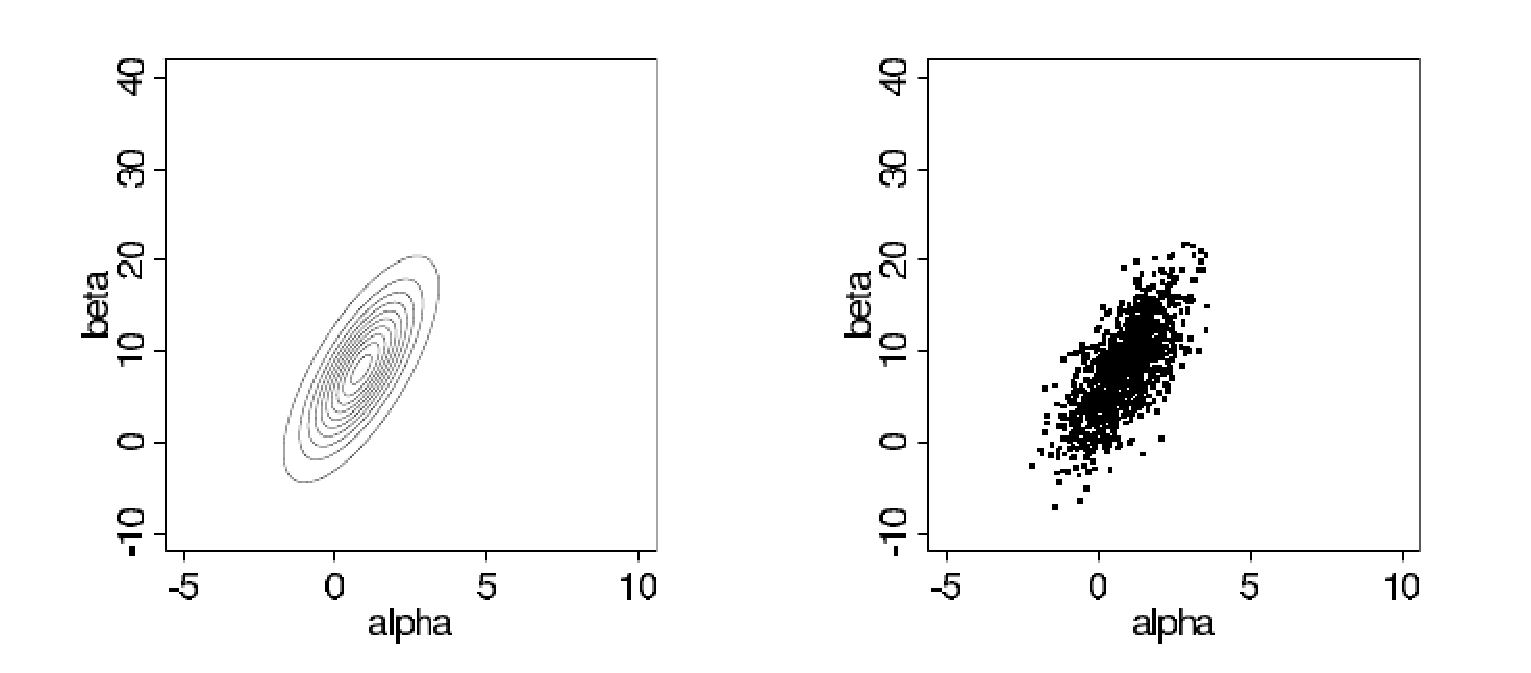
\includegraphics[scale = 0.45]{pictures/fig_4_1.eps}
\caption{Výsledky biotestu - (a) konturový graf, (b) korelační graf}
\label{fig_4_1}
\end{figure}

\subparagraph{Aposteriorní rozdělení LD50 s využitím normální aproximace parametrů $(\alpha, \beta)$.}

Výběr 1~000 pozorování náhodně vygenerovaných z normální aproximace aposteriorního rozdělení lze použít také pro odhad pravděpodobnosti $p(\beta > 0)$ a LD50 podmíněně na $\beta > 0$. Z 1~000 pozorování již 950 splňuje $\beta > 0$.
\begin{figure}[htp]
\centering
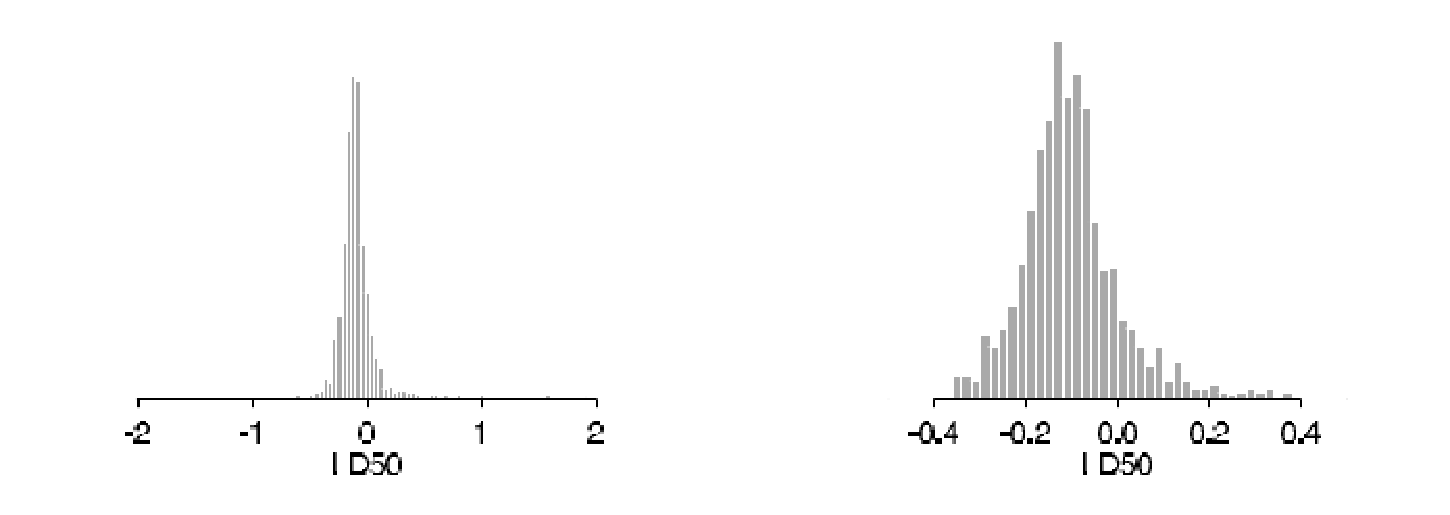
\includegraphics[scale = 0.45]{pictures/fig_4_2.eps}
\caption{Výsledky biotestu - (a) konturový graf, (b) korelační graf}
\label{fig_4_2}
\end{figure}
Obrázek 4.2a ilustruje histogram LD50 hodnot bez některých extrémních hodnot v obou chvostech.\footnote{Pokud bychom extrémní hodnoty v grafu ponechali, bylo by jeho měřítko zdeformované do té míry, že by byl nečitelný.} Obrázek 4.2b pak představuje výřez z 4.2a v okolí módu. Oba histogramy jsou centrovány přibližně kolem stejného bodu jako 3.3, nicméně vykazují mnohem vyšší volatilitu a to z důvodu vyšší pravděpodobnosti, že je skutečná hodnota parametru $\beta$ blízká nule.

Aposteriorní rozdělení založené na normální aproximaci je tedy podobné skutečnému aposteriornímu rozdělení. Nicméně, s ohledem na malou velikost náhodného výběru, je skutečné aposteriorní rozdělení výrazně více sešikmené než jeho normální aproximace, která je založená na předpokladu náhodného výběru velkého rozsahu. Proto má skutečné aposteriorní rozdělení LD50 mnohem kratší chvosty než je tomu v případě aposteriorního rozdělení založeného na normální aproximaci.

\section{Výběr velkého rozsahu}

\subsection{Úvod do problematiky}

Základním nástrojem Bayesiánské inference pro výběry velkého rozsahu je předpoklad asymptotické normality aposteriorního rozdělení. Asymptotická normalita je založena na myšlence, že s tím, jak podkladový proces generuje stále více nových dat, se aposteriorní rozdělení parametrového vektoru $\theta$ stále více blíží vícerozměrnému normálnímu rozdělení, i když skutečné pravděpodobností rozdělení dat nespadá pod uvažovanou parametrickou rodinu pravděpodobnostních rozdělení. Tento závěr lze nejsnáze aplikovat na pozorování $y_1, ..., y_n$, která jsou nezávislá a pocházejí ze společného pravděpodobnostního rozdělení $f(y)$.

Předpokládejme, že data jsou modelována pomocí parametrické rodiny $p(y|\theta)$ s apriorním rozdělením $p(\theta)$.  Jestliže je skutečné pravděpodobnostní rozdělení dat pokryté uvažovanou parametrickou rodinou, tj. jestliže $f(y) = p(y|\theta_0)$ pro určité $\theta_0$, pak je díky asymptotické normalitě splněn předpoklad konzistence. To znamená, že aposteriorní rozdělení konverguje k bodu, který představuje skutečnou hodnotu parametru $\theta_0$ s tím, jak $n \rightarrow \infty$. Pokud skutečné rozdělení uvažovanou parametrickou rodinou pokryté není, skutečné hodnoty $\theta_0$ nemusí být dosaženo - její roli přebírá hodnota $\theta_0$, pro kterou je rozdělení $p(y|\theta)$ nejbližší skutečnému rozdělení $f(y)$.

\subsection{Asymptotická normalita a konzistence}

Lze dokázat, že při splnění určitých předpokladů\footnote{Zejména se jedná o předpoklad, že věrohodnostní funkce je spojitá funkce v parametru $\theta$ a že $\theta_0$ neleží na hranici parametrového prostoru.} se aposteriorní rozdělení parametru $\theta$ blíží normálnímu rozdělení se střední hodnotu $\theta_0$ a rozptylem $\big(nJ(\theta_0)\big)^{-1}$ s tím, jak $n \rightarrow \infty$. Zjednodušeně lze tento závěr chápat v kontextu Taylorova rozvoje (4.1) logaritmu aposteriorní hustoty centrované na aposteriorní mód $\hat{\theta}$. Lze dokázat, že aposteriorní mód $\hat{\theta}$ je konzistentním odhadem skutečné hodnoty parametru $\theta_0$, tj. že a aposteriorní rozdělení $p(\theta|y)$ se koncentruje stále více a více kolem $\theta_0$ a že vzdálenost $|\hat{\theta} - \theta_0|$ se blíží nule s tím, jak $n \rightarrow \infty$.

S pomocí $p(\theta|y) = p(\theta) p(y|\theta)$ můžeme kvadratický člen (4.1) přepsat do tvaru
\begin{equation}
\Big[\frac{d^2}{d \theta^2} \ln\big(p(\theta|y)\big)\Big]_{\theta = \hat{\theta}} = \Big[\frac{d^2}{d \theta^2} \ln\big(p(\theta)\big)\Big]_{\theta = \hat{\theta}} + \sum_{i = 1}^n \Big[\frac{d^2}{d \theta^2} \ln\big(p(y_i|\theta)\big)\Big]_{\theta = \hat{\theta}}.
\end{equation}
Na tento člen, který je funkcí parametru $\theta$, lze nahlížet jako na součet konstanty a sumy $n$ členů, jejichž střední hodnota je pro skutečnou výběrovou distribuci $p(y|\theta)$ přibližně $-J(\theta_0)$, pokud je aposteriorní mód $\hat{\theta}$ dostatečně blízko skutečné hodnotě parametru $\theta_0$.\footnote{Předpokládáme, že $f(y) = p(y|\theta_0)$ pro určitou hodnotu $\theta_0$.} Proto lze pro velká $n$ aproximovat sešikmení logaritmu aposteriorního rozdělení Fisherovou informací v bodě $\hat{\theta}$.

Výše uvedené lze shrnout tak, že v kontextu zvolené pravděpodobnostní rodiny se pro velká $n$ (a) aposteriorní mód $\hat{\theta}$ limitně blíží skutečné hodnotě $\theta_0$ uvažovaného parametru a (b) sešikmení aposteriorního rozdělení se blíží $nJ(\hat{\theta})$. Dále platí, že pro $n \rightarrow \infty$ dominuje věrohodnostní funkce nad apriorním rozdělením, a proto lze použít pouze věrohodnostní funkci, abychom získali mód a sešikmení pro účely konstrukce normální aproximace.

\subsection{Dominance věrohodnostní funkce nad apriorním rozdělením}

Výše popsaná asymptotická vlastnost dává za pravdu intuici, že význam apriorního rozdělení klesá s tím, jak se zvětšuje velikost vzorku. Logickým důsledkem tohoto závěru je, že si v případě, kdy máme k dispozici velké množství dat, nemusíme příliš lámat hlavu s formulací apriorního rozdělení. A naopak, pokud je vzorek relativně malý, může hrát volba apriorního rozdělení velmi důležitou úlohu.

\section{Nesplnění předpokladů normální aproximace}

Pro níže uvedené případy nejsou splněny předpoklady normální aproximace, a proto má v jejich případě volba apriorního rozdělení vliv na aposteriorní inference, a to i v případě výběrů velkého rozsahu.

\subsection{Nedostatečně identifikované modely}

O modelu říkáme, že je nedostatečně identifikován, pokud je jeho věrohodnostní funkce $p(\theta|y)$ konstantní pro určité rozmezí hodnot parametru $\theta$. Pro takovéto modely neexistuje jediný bod $\theta_0$, ke kterému by aposteriorní rozdělení mohlo konvergovat.

\subsection{Nedostatečně identifikované parametry}

Uvažujme model
\begin{equation}
\begin{bmatrix}u \\ v \end{bmatrix} \sim N \Big(\begin{bmatrix}0 \\ 0 \end{bmatrix}, \begin{bmatrix} 1 & \rho\\ \rho & 1 \end{bmatrix} \Big),
\end{equation}
ve kterém je pro každý pár $(u, v)$ pozorováno pouze $u$ nebo $v$. V tomto případě je parametr $\rho$ neidentifikovaný. Pozorovaná data nám totiž neposkytují žádnou informaci o $\rho$, a proto je aposteriorní rozdělení tohoto parametru stejné bez ohledu na počet pozorování jako jeho apriorní rozdělení.

\subsection{Počet parametrů narůstá s velikostí výběru}

Pokud počet parametrů narůstá s počtem pozorování, pak výše uvedené závěry, které předpokládají fixní model $p(y_i | \theta)$, neplatí. Pro ilustraci uvažujme situaci, kdy je každému pozorování přiřazen parametr - např. $y_i \sim N(\theta_i, \sigma^2)$. Obecně platí, že parametry $\theta_i$ nelze konzistentně odhadnout, pokud se objem dat pro každé pozorování nezvyšuje ruku v ruce s počtem jednotek $i$.

Stejně jako v případě nedostatečně identifikovaných modelů nebude aposteriorní rozdělení parametru $\theta_i$ konvergovat k jeho skutečné hodnotě, pokud nová data nepřinesou také novou informaci o $\theta_i$. V tomto konkrétním případě aposteriorní rozdělení nekonverguje k určitému bodu, protože parametrický prostor neustále narůstá v důsledku zvyšující se dimensionality parametru $\theta$.

\subsection{Zaměnitelné parametry}

Uvažujme směsný normální model s nezávislými daty $y_1, ..., y_n$ z identického pravděpodobnostního rozdělení a parametrickým vektorem $\theta = (\mu_1, \mu_2, \sigma_1^2, \sigma_2^2, \lambda)$, kde
\begin{equation}
p(y_i|\mu_1, \mu_2, \sigma_1^2, \sigma_2^2, \lambda) = \lambda \frac{1}{\sqrt{2 \pi} \sigma_1}e^{-\frac{1}{2 \sigma_1^2}(y_i - \mu_1)^2} + (1 - \lambda) \frac{1}{\sqrt{2 \pi} \sigma_2}e^{-\frac{1}{2 \sigma_2^2}(y_i - \mu_2)^2}.
\end{equation}
Pokud prohodíme hodnoty v párech $(\mu_1, \mu_2)$ a $(\sigma_1^2, \sigma_2^2)$ a vyměníme $\lambda$ za $(1 - \lambda)$, nebude to mít vliv na věrohodnostní funkci. Aposteriorní rozdělení takovéhoto modelu tak má alespoň dva módy a skládá se ze dvou rozdělení, která jsou vzájemně zrcadlová, a proto nekonverguje do jednoho bodu a to bez ohledu na počet pozorování. Tento problém lze odstranit omezením parametrického prostoru tak, abychom odstranili případné duplicity - např. v našem případě lze parametrický prostor omezit podmínkou $\mu_1 \le \mu_2$.

\subsection{Neohraničená věrohodnostní funkce}

Jestliže je věrohodnostní funkce neohraničená (unbounded), pak v rámci parametrického prostoru nemusí existovat aposteriorní mód, což je v rozporu s předpokladem normální aproximace. Pro ilustraci uvažujme předchozí směsný normální model. Pro zjednodušení předpokládejme, že $\lambda$ je známá hodnota z otevřeného intervalu $(0, 1)$. Jestliže $\mu_1 = y_i$ pro arbitrárně zvolené $y_i$ a $\sigma_1^2 \rightarrow 0$, pak se věrohodnostní funkce blíží nekonečnu. Jak se $n$ blíží nekonečnu, narůstá počet módu věrohodnostní funkce. Jestliže je apriorní rozdělení parametru $\sigma_1^2$ uniformní a $\sigma_2^2$ se nachází poblíž nuly, narůstá také počet módů aposteriorního rozdělení, pro které neexistují odpovídající normální aproximace. Pokud je apriorní rozdělení proporcionální k $\frac{1}{\sigma_1^2 \sigma_2^2}$, je více pravděpodobnostní masy koncentrováno v okolí nuly, což má za následek ještě větší `explozi' aposteriorního rozdělení v tomto bodě.

K výše popsané situaci však v praxi dochází pouze zřídka, protože neohraničená věrohodnostní funkce je často důsledkem nerealistických podmínek v rámci modelu.

\subsection{Nevlastní aposteriorní rozdělení}

Uvažujme nenormalizované aposteriorní rozdělení získané vynásobením věrohodnostní funkce `formálním' nevlastním apriorním rozdělením. Pokud je integrál tohoto aposteriorní rozdělení roven nekonečnu, není splněn předpoklad asymptoticky normálního rozdělení, který je založen na předpokladu, že součet pravděpodobností je roven nule.

Připomeňme, že nevlastní aposteriorní rozdělení nemůže vzniknout jinak než v důsledku nevlastního apriorního rozdělení. Řešení problému je snadné - pokud zvolené apriorní rozdělení nevede k vlastnímu aposteriornímu rozdělení, je třeba zvolit jiné apriorní rozdělení, tak aby byl integrál výsledného aposteriorního rozdělení konečný.

\subsection{Apriorní rozdělení, které nezahrnuje konvergenční bod}

Jestliže $p(\theta_0) = 0$ pro nespojitý parametrický prostor nebo $p(\theta_0) = 0$ v okolí $\theta_0$ pro spojitý parametrický prostor, pak není splněn předpoklad konvergence, který je založen na dominanci věrohodnostní funkce nad apriorním rozdělením. Řešením je přiřadit všem myslitelným hodnotám parametru $\theta$ nenulovou hodnotu.

\subsection{Konvergence k hranici parametrického prostoru}

Jestliže se skutečná hodnota $\theta_0$ hledaného parametru $\theta$ nachází na hranici parametrického prostoru, pak musí být Taylorův rozvoj v daném směru `odseknutý' a výsledná normální aproximace tak nemusí být aplikovatelná a to ani v případě výběru velkého rozsahu.

Pro ilustraci uvažujme model $y_i \sim N(\theta, 1)$ s omezením $\theta \ge 0$. Předpokládejme, že se jedná o přesný model se skutečnou hodnotou parametru $\theta = 0$. Aposteriorní rozdělení parametru $\theta$ je normální centrované na $\overline{y}$ s `odseknutou' zápornou částí. Aposteriorní rozdělení parametru $\theta$ má tak pro $n \rightarrow \infty$ tvar polovičního normálního rozdělení centrovaného na bodě nula.

Uvažujme výše uvedený model, avšak tentokrát předpokládejme skutečnou hodnotu parametru $\theta = -1$, tj. hodnotu mimo parametrický prostor. Limitní aposteriorní rozdělení parametru $\theta$ má ostré maximum v bodě nula, však jeho tvar nebude ani vzdáleně připomínat tvar normálního rozdělení.

Řešením popsaného problému je uvědomit si, že se skutečná hodnota parametru nachází na hranici nebo dokonce za hranicí uvažovaného parametrického prostoru. Z tohoto důvodu je vhodné přiřadit všem myslitelným hodnotám parametru $\theta$ nenulovou pravděpodobnost.

\subsection{Chvosty pravděpodobnostního rozdělení}

Normální aproximace je často přijatelná pro většinu pravděpodobnostní masy aposteriorního rozdělení s výjimkou chvostů. Uvažujme situaci, kdy je $p(\theta | y)$ proporcionální k $e^{-c|\theta|}$ s tím, jak se $|\theta|$ blíží k nekonečnu, kde $c$ představuje konstantu.\footnote{Pro srovnání, normální rozdělení je proporcionální k $e^{-c\theta^2}$.} Pravděpodobnostní rozdělení stále konverguje k normálnímu rozdělení, avšak pro libovolný konečný vzorek velikosti $n$ tato aproximace selhává ve chvostech.

Jako další příklad uvažujme situaci, kdy je parametr $\theta$ omezený na kladné hodnoty. Pro libovolný konečný výběr bude normální aproximace přiřazovat nenulovou pravděpodobnost záporné hodnotě parametru, což je v rozporu se skutečným stavem věci.

\section{Bayesiánské inference}

\subsection{Shoda ve výběrech velkého rozsahu}

Předpokládejme, že lze aposteriorní rozdělení parametru $\theta$ aproximovat normálním rozdělením pomocí (4.2). Pak můžeme aplikovat transformaci
\begin{equation}
[I(\hat{\theta})]^{1/2}(\theta - \hat{\theta})|y \sim N(0, I),
\end{equation}
kde $\hat{\theta}$ je aposteriorní mód a $[I(\hat{\theta})]^{1/2}$ je libovolný kořen čtvercové matice $I(\hat{\theta})$. Navíc, protože $\hat{\theta} \rightarrow \theta_0$, můžeme výše uvedenou aproximaci vyjádřit pomocí $I(\theta_0)$. Jestliže je skutečné pravděpodobnostní rozdělení dat zahrnuto v uvažované třídě modelů, tj. $f(y) \equiv p(y|\theta)$ pro určité $\theta$, pak lze pro opakovaný výběr s fixním $\theta$ dokázat, že pro $n \rightarrow \infty$ platí
\begin{equation}
[I(\hat{I})]^{1/2}(\theta - \hat{\theta}) | \theta \sim N(0, I).
\end{equation}
Jedná se o závěr klasické statistické teorie, který je platný pro hodnotu odhadu $\hat{\theta}$ získaného metodou maximální věrohodnosti. Tento závěr lze snadno rozšířit také na situace, kdy je $\hat{\theta}$ rovno aposteriornímu módu. Výše uvedené výsledky implikují, že pro libovolnou funkci $(\theta - \hat{\theta})$ je aposteriorní rozdělení odvozené z (4.16) asymptoticky totožné s rozdělením získaným opakovaným výběrem z (4.17). To znamená, že 95\% aposteriorní interval parametru $\theta$ bude v 95\% případů opakovaného náhodného výběru obsahovat skutečnou hodnotu $\theta_0$.

\subsection{Bodový odhad, konzistence a efektivita odhadu}

Bodový odhad parametru $\theta$ dává smysl především v případě výběru velkého rozsahu, kdy je aposteriorní mód $\hat{\theta}$ `centrem' aposteriorního rozdělení parametru $\theta$ a nejistota reprezentovaná $nI(\hat{\theta})$ je relativně zanedbatelná. Nicméně pro výběry malého rozsahu bodový odhad parametru $\theta$ příliš smysl nedává - mnohem vhodnější je presentovat celé jeho aposteriorní rozdělení popř. hodnoty vybraných kvantilů.

O bodovém odhadu říkáme, že je konzistentní, pokud konverguje k správné hodnotě parametru s tím, jak roste velikost vzorku. Proto, pokud $f(y) \equiv p(y|\theta_0)$, je bodový odhad $\hat{\theta}$ parametru $\theta$ konzistentní, pokud jeho výběrové rozdělení konverguje k bodu $\theta_0$ s tím, jak roste velikost výběru $n$. Blízký koncept je pak tzv. asymptotická nezkreslenost, kde $\frac{E(\hat{\theta}|\theta_0)}{sd(\hat{\theta}|\theta_0)}$ konverguje k nule.\footnote{$\hat{\theta}(y)$ opět považujeme za náhodnou veličinu, jejíž pravděpodobnostní rozdělení je dáno $p(y|\theta_0)$.} Pokud rodina modelů, které kalibrujeme na pozorovaných datech, je zahrnuje skutečné pravděpodobnostní rozdělení, pak je nejen aposteriorní mód $\hat{\theta}$ ale také aposteriorní střední hodnota a medián konzistentní a asymptoticky nezkreslený a to při splnění několika relativně neomezujících regulárních podmínek.

O bodovém odhadu říkáme, že efektivní, pokud neexistuje žádná další funkce parametru $y$, která by odhadovala hodnotu parametru $\theta$ s nižší směrodatnou odchylkou, tj. $E\big((\hat{\theta} - \theta_0)^2 | \theta_0 \big)$ je nejnižší dosažitelná (aka optimální) hodnota. Efektivita odhadu $\hat{\theta}$ se měří jako poměr optimální směrodatné odchylky a skutečné směrodatné odchylky odhadu $\hat{\theta}$. Odhad je asymptoticky efektivní, pokud se tento poměr blíží jedné s tím, jak se velikost výběru $n$ blíží nekonečnu. Při splnění několika neomezujících regulárních podmínek je `střed' aposteriorního rozdělení (definovaný např. jako aposteriorní střední hodnota, medián nebo mód) asymptoticky efektivní.

\subsection{Interval spolehlivosti}

Jestliže region $C(y)$ zahrnuje $\theta_0$ v alespoň $100(1 - \alpha)\%$ případech opakovaných výběrů, pak $C(y)$ nazýváme $100(1 - \alpha)\%$ intervalem spolehlivosti parametru $\theta$. Pro ilustraci si připomeňme, že v předchozím textu jsme tvrdili, že $100(1 - \alpha)\%$ aposteriorní interval parametru $\theta$ má tu asymptotickou vlastnost, že pro opakované náhodné výběry $y$ obsahuje $100(1 - \alpha)\%$ intervalů hodnotu $\theta_0$.

\section{Bayesiánská interpretace ostatních statistických metod}

\subsection{Metoda maximální věrohodnosti a další bodové odhady}

Z pohledu Bayesiánské analýzy dat lze klasický bodový odhad často interpretovat jako aposteriorní statistiku založenou na implicitním pravděpodobnostním modelu. V případě výběru velkého rozsahu lze dokonce obhájit klasickou metodu maximální věrohodnosti pomocí Bayesiánského přístupu. Při splnění regulárních podmínek je totiž v limitě $n \rightarrow \infty$ odhad $\hat{\theta}$ získaný metodou maximální věrohodnosti  dostatečnou statistikou stejně jako aposteriorní mód, střední hodnota či medián. Jinými slovy, pro dostatečně veliké $n$ obsahuje odhad založený na metodě maximální věrohodnosti stejnou informaci o hledaném parametru $\theta$ jako samotná data.

V případě opakovaného náhodného výběru s $\theta = \theta_0$ platí
\begin{equation}
p \big(\hat{\theta}|\theta = \theta_0 \big) \approx N\big(\hat{\theta}(y)|\theta_0, (nJ(\theta_0))^{-1}\big).
\end{equation}
Výběrové rozdělení náhodné veličiny $\hat{\theta}(y)$ je tedy přibližně normální se střední hodnotou $\theta_0$ a přesností $nJ(\theta_0)$.\footnote{Abychom předešli nedorozumění, zápisem $\hat{\theta}(y)$ zdůrazňujeme, že $\hat{\theta}$ je funkcí $y$.} Pokud budeme předpokládat, že apriorní rozdělení je lokálně uniformní (nebo spojité a nenulové) v okolí skutečné hodnoty parametru $\theta$, pak prostá analýza normální střední hodnoty (viz. sekce 3.5) implikuje, že aposteriorní Bayesiánská inference má podobu
\begin{equation}
p(\theta | \hat{\theta}) \approx N(\theta | \hat{\theta}, (nJ(\hat{\theta}))^{-1}).
\end{equation}
Tento závěr přímo vyplývá z asymptotické normality, nicméně jeho odvození nepřímo skrze Bayesiánskou inferenci má poskytuje vhled do Bayesiánského odůvodnění klasické asymptotické inference založené na bodových odhadech a směrodatných odchylkách.

Závěrem připomeňme, že pro konečné $n$ není výše uvedený přístup efektivní, protože $\hat{\theta}$ není dostatečnou statistikou.

\subsection{Nezkreslené odhady}

Některé statistické metody kladou velký důraz na nezkreslenost odhadů. Odhad $\theta | y$ nazýváme nezkresleným, jestliže $E\big(\hat{\theta}(y)|\theta\big) = \theta$ pro libovolné $\theta$, kde tato střední hodnota je vypočtena pomocí $p(y|\theta)$. Z pohledu Bayesiánského přístupu je požadavek na nezkreslenost rozumný v limitě pro výběry velkého rozsahu nicméně potenciálně zavádějící v ostatních případech. Minimalizace zkreslení totiž v praxi často vede k nežádoucímu nárůstu rozptylu daného odhadu.

Obecný problém požadavku na nezkreslenost je, že v praxi je často nemožné odhadnout několik parametrů najednou tak, aby byly alespoň `přibližně' nezkreslené.

\subsubsection{Ilustrativní příklad - predikce pomocí regrese}

Nechť parametr $\theta$ představuje výšku dospělé dcery při známé výšce $y$ její matky. Předpokládejme, že výška dcery a matky sledují sdružené normální rozdělení se střední hodnotou 160 centimetrů, shodnou směrodatnou odchylkou a korelací 0.50. Aposteriorní střední hodnota parametru $\theta$ má tedy tvar
\begin{equation}
E(\theta | y) = 160 + 0.5(y - 160).
\end{equation}
Aposteriorní střední hodnota však není nezkresleným odhadem parametru $\theta$ ve smyslu opakovaného výběru $y$ pro fixované $\theta$. Pro danou výšku dcery $\theta$ má výška matky $y$ střední hodnotu $E(y | \theta) = 160 + 0.50(\theta - 160)$. Proto je v případě opakovaného výběru $y$ při fixovaném $\theta$ aposteriorní střední hodnota rovna $160 + 0.25(\theta - 160)$ a je zkreslená směrem ke střední hodnotě 160. Naopak podmíněný odhad
\begin{equation}
\hat{\theta} = 160 + 2(y - 160)
\end{equation}
je nezkreslený pro opakovaný výběr $y$. Odhad $\hat{\theta}$ bohužel nedává smysl pro hodnoty $y$ různé od 160. Pokud je matka např. o 10 centimetrů vyšší než průměrně vysoká žena, je dle tohoto odhadu její dcera o 20 centimetrů vyšší než průměr.

V tomto jednoduchém případě, ve kterém parametr $\theta$ sleduje zvolené populační rozdělení, by nebayesiánský statistik nepoužil $\hat{\theta}$ jako nezkreslený odhad. Namísto toho by tento problém `překlasifikoval' jako predikci.

\subsection{Intervaly spolehlivosti}

I pro výběry malého rozsahu jsou Bayesiánské $(1 - \alpha)\%$ aposteriorní intervaly spolehlivosti často blízké $(1 - \alpha)\%$ intervalům spolehlivosti pro opakované výběry podmíněné $\theta$. Nicméně existují intervaly spolehlivosti, které jsou založeny čistě na teorii výběru, a které jsou zcela odlišné od Bayesiánských pravděpodobnostních intervalů. Mnoho autorů ukázalo, že obecná teorie založená na nepodmíněném chování může často vést k neintuitivním výsledkům, jako jsou intervaly s nulovou nebo nekonečnou délkou. Jako jednoduchý příklad lze uvést interval spolehlivost, který je v 5\% případů prázdný a v 95\% případů obsahuje všechna reálná čísla. Tím je zajištěno, že tento interval v 95\% případů zahrnuje skutečnou hodnotu parametru $\theta$, protože v 95\% případů zahrnuje všechna reálná čísla. Tento příklad nemá za cíl zpochybnit přínos intervalů spolehlivosti, ale spíše ukázat, že samotná konvergence nezaručuje smysluplné inference.

\subsection{Testování hypotéz}

Pokud má Bayesiánská analýza vést k nenulové aposteriorní pravděpodobnosti pro nulovou hypotézu o bodovém odhadu, musíme nejprve formulovat apriorní rozdělení daného parametru tak, aby apriorní pravděpodobnost platnosti této hypotézy byla také nenulová. V případě spojitého parametru lze takové apriorní rozdělení nalézt poměrně snadno. Největší problémy s interpretací výsledků testování hypotéz je obvykle dáno formulací nulové resp. alternativní hypotézy ve tvaru $H_0: \theta = \theta_0$ resp. $H_1: \theta \ne \theta_0$. V případě spojitého parametru $\theta$ (definovaného např. jako rozdíl dvou středních hodnot) nedává nulová hypotéza $H_0: \theta = 0$ povětšinou příliš smysl a spíše nás zajímá pravděpodobnostní rozdělení popř. odpovídající interval odhadu parametru $\theta$.

Řada jednoduchých testů může být chápána jako analogie aposteriorní pravděpodobnosti pro neinformativní apriorní rozdělení. Např. předpokládejme, že pozorujeme $y = 1$ z modelu $y \sim N(\theta, 1)$ s apriorním uniformním rozdělením pro parametr $\theta$. Nemůžeme zamítnout hypotézu $\theta = 0$, protože jednostranná $p$-hodnota je 0.16 a dvoustranná $p$-hodnota je 0.32, tj. v obou případech vyšší než obvyklá hraniční hodnota 0.05. Na druhou stranu, pravděpodobnost $\theta > 0$ je 84\%, což je více informativní údaj než pouhý verdikt o zamítnutí či nezamítnutí nulové hypotézy.

\subsection{Vzájemné porovnání vícero parametrů}

Uvažujme nezávislá měření $y_j \sim N(\theta_j, 1)$ pro každý z $J$ parametrů, jejichž cílem je kvantifikovat rozdíly a pořadí spojitých parametrů $\theta_j$. V klasické statistice se nabízí několik metod víceúrovňového porovnání, které testují, zda-li jsou jednotlivá $\theta_j$ `významně' odlišná. V případě Bayesiánského přístupu sledují parametry $\theta_j$ sdružené pravděpodobnostní rozdělení. S jeho pomocí tak můžeme (alespoň teoreticky) určit aposteriorní pravděpodobnost každého z $J!$ možných pořadí.